% exercise sheet with header on every page for math or close subjects
\documentclass[12pt]{article}
\usepackage[utf8]{inputenc} 
\usepackage{latexsym} 
\usepackage{multicol}
\usepackage{fancyhdr}
\usepackage{amsfonts} 
\usepackage{amsmath}
\usepackage{amssymb}
\usepackage{enumerate}
\usepackage{listings}
\usepackage{graphicx}

% Shortcuts for bb, frak and cal letters
\newcommand{\E}{\mathbb{E}}
\newcommand{\V}{\mathbb{V}}
\renewcommand{\P}{\mathbb{P}}
\newcommand{\N}{\mathbb{N}}
\newcommand{\R}{\mathbb{R}}
\newcommand{\C}{\mathbb{C}}
\newcommand{\Z}{\mathbb{Z}}
\newcommand{\Pfrak}{\mathfrak{P}}
\newcommand{\Pfrac}{\mathfrak{P}}
\newcommand{\Bfrac}{\mathfrak{P}}
\newcommand{\Bfrak}{\mathfrak{B}}
\newcommand{\Fcal}{\mathcal{F}}
\newcommand{\Ycal}{\mathcal{Y}}
\newcommand{\Bcal}{\mathcal{B}}
\newcommand{\Acal}{\mathcal{A}}

% formating
\topmargin -1.5cm 
\textheight 24cm
\textwidth 16.0 cm 
\oddsidemargin -0.1cm

% Fancy Header on every Page
\pagestyle{fancy}
\lhead{\textbf{Pattern and Speech Recognition}}
\rhead{Daniel Schäfer (2549458)\\ Christian Bohnenberger (2548364) \\ Dominik Weber (2548553)}
\renewcommand{\headrulewidth}{1.2pt}

\setlength{\headheight}{45pt} 

\begin{document}
\pagenumbering{gobble}

% TODO set the number of the exercise sheet here!
\setcounter{section}{2}

\subsection{PCA}
\begin{enumerate}[a)]
    \item 
        % TODO
        $$X =\begin{bmatrix} 1&1 \\ 2&2 \\ 3 & 1 \\ 4 & 1 \end{bmatrix}$$\\
        $X$ with mean $0$:\\
        $$X =\begin{bmatrix} -\frac{3}{2}& -\frac{1}{4} \\ -\frac{1}{2}&\frac{3}{4} \\ \frac{1}{2} & -\frac{1}{4} \\ \frac{3}{2} & -\frac{1}{4} \end{bmatrix}$$\\
        We continue with the matrix with mean zero.\\
        $$X^T * X = \begin{bmatrix} -\frac{3}{2}& -\frac{1}{2} & \frac{1}{2} & \frac{3}{2} \\
        				-\frac{1}{4} & \frac{3}{4} & -\frac{1}{4}  & -\frac{1}{4} \end{bmatrix} *
        				\begin{bmatrix} -\frac{3}{2}& -\frac{1}{4} \\ -\frac{1}{2}&\frac{3}{4} \\ \frac{1}{2} & -\frac{1}{4} \\ \frac{3}{2} & -\frac{1}{4} \end{bmatrix} 
        				= \begin{bmatrix}
        					5 & -0.5 \\
        					-0.5 & 3
        				\end{bmatrix}
        				$$\\
        	Now we can compute the eigenvalues:\\
        		$$ (5 - \lambda)*(3 - \lambda)-0.25 =0$$\\
        		$$ 15 - 8\lambda + \lambda^2 -0.25 = 0$$\\
        		$$ \Rightarrow \lambda_1= 2.88197, \lambda_2=5.11803 $$\\
        		
        		$$ \begin{bmatrix} 5-5.11803 & -0.5 \\ -0.5 & 3-5.11803 \end{bmatrix}* \begin{bmatrix} x_1 \\ x_2 \end{bmatrix}
        		=\begin{bmatrix} 0 \\ 0 \end{bmatrix} $$\\
        		$$ \Rightarrow -\frac{1}{2}*x_1 - 2.11803*x_2= 0 $$\\ 
        		$$ \Rightarrow  \text{eigenvector:}  \begin{bmatrix} 4.23606 \\ 1 \end{bmatrix} $$\\
        		$$ D= \begin{bmatrix} 4.23606 \\ 1 \end{bmatrix} $$\\
        		Encoder: $f(x)= D^T * x$\\
        		Decoder: $g(x)= D* D^T *x$\\
        		Encoding:\\
        		\begin{itemize}
        			\item $f(x^{(1)})= \begin{bmatrix} 4.23606, & 1 \end{bmatrix} * \begin{bmatrix} 1 \\ 1 \end{bmatrix} = 5.23606$
        			\item $f(x^{(2)})= \begin{bmatrix} 4.23606, & 1 \end{bmatrix} * \begin{bmatrix} 2 \\ 2 \end{bmatrix} = 10.47212$
        			\item $f(x^{(3)})= \begin{bmatrix} 4.23606, & 1 \end{bmatrix} * \begin{bmatrix} 3 \\ 1 \end{bmatrix} = 13.70818$
        			\item $f(x^{(4)})= \begin{bmatrix} 4.23606, & 1 \end{bmatrix} * \begin{bmatrix} 4 \\ 1 \end{bmatrix} = 17.94424$
        		\end{itemize}
        		Decoding:$D*D^T*x$ ($D^T*x$ is already computed)\\
        		\begin{itemize}
        			\item $\begin{bmatrix} 4.23606, & 1  \end{bmatrix}*5.23606= \begin{bmatrix} 22.18026 \\7.61623 \end{bmatrix}$
        			\item $\begin{bmatrix} 4.23606, & 1  \end{bmatrix}*10.47212= \begin{bmatrix} 44.36053 \\10.47212  \end{bmatrix}$ 
        			\item $\begin{bmatrix} 4.23606, & 1  \end{bmatrix}*13.70818= \begin{bmatrix} 58.06867297 \\ 13.70818 \end{bmatrix}$ 
        			\item $\begin{bmatrix} 4.23606, & 1  \end{bmatrix}*17.94424= \begin{bmatrix} 76.01287729 \\ 17.94424 \end{bmatrix}$  
        		\end{itemize}
        		\newpage
    \item
        % TODO
        $$X =\begin{bmatrix} -1&1 \\ -2&2 \\ -1 & 3 \\ -1 & 4 \end{bmatrix}$$\\
        $X$ with mean $0$:\\
        $$X =\begin{bmatrix} \frac{1}{4}& -\frac{3}{2} \\ -\frac{3}{4}&-\frac{1}{2} \\ \frac{1}{4} & \frac{1}{2} \\ \frac{1}{4} & \frac{3}{2} \end{bmatrix}$$\\
        We continue with the matrix with mean zero.\\
        $$X^T * X = \begin{bmatrix} \frac{1}{4} & -\frac{3}{4} & \frac{1}{4}  & \frac{1}{4}\\
        				-\frac{3}{2}& -\frac{1}{2} & \frac{1}{2} & \frac{3}{2} \\
        				\end{bmatrix} *
        				\begin{bmatrix} \frac{1}{4}& -\frac{3}{2} \\ -\frac{3}{4}&-\frac{1}{2} \\ \frac{1}{4} & \frac{1}{2} \\ \frac{1}{4} & \frac{3}{2} \end{bmatrix}
        				= \begin{bmatrix}
        					0.75 & 0.5 \\
        					0.5 & 5
        				\end{bmatrix}
        				$$\\
        	Now we can compute the eigenvalues:\\
        		$$ (0.75 - \lambda)*(5 - \lambda)-0.25 =0$$\\
        		$$ 3.75 - 5.75\lambda + \lambda^2 -0.25 = 0$$\\
        		$$ \Rightarrow \lambda_1= 0.691969, \lambda_2=5.05803 $$\\
        		
        		$$ \begin{bmatrix} 0.75-5.05803 & 0.5 \\ 0.5 & 5-5.05803 \end{bmatrix}* \begin{bmatrix} x_1 \\ x_2 \end{bmatrix}
        		=\begin{bmatrix} 0 \\ 0 \end{bmatrix} $$\\
        		$$ \Rightarrow \frac{1}{2}*x_1 - 0.05803*x_2= 0 $$\\ 
        		$$ \Rightarrow  \text{eigenvector:}  \begin{bmatrix} 1 \\ 8.61623 \end{bmatrix} $$\\
        		$$ D= \begin{bmatrix} 1 \\ 8.61623 \end{bmatrix} $$\\
        		Encoder: $f(x)= D^T * x$\\
        		Decoder: $g(x)= D* D^T *x$\\
        		Encoding:\\
        		\begin{itemize}
        			\item $f(x^{(1)})= \begin{bmatrix} 1 & 8.61623  \end{bmatrix} * \begin{bmatrix} -1 \\ 1 \end{bmatrix} = 7.61623$
        			\item $f(x^{(2)})= \begin{bmatrix} 1 & 8.61623  \end{bmatrix} * \begin{bmatrix} -2 \\ 2 \end{bmatrix} = 15.23246$
        			\item $f(x^{(3)})= \begin{bmatrix} 1 & 8.61623  \end{bmatrix} * \begin{bmatrix} -1 \\ 3 \end{bmatrix} = 24,84869$
        			\item $f(x^{(4)})= \begin{bmatrix} 1 & 8.61623  \end{bmatrix} * \begin{bmatrix} -1 \\ 4 \end{bmatrix} = 33.46492$
        		\end{itemize}
        		Decoding:$D*D^T*x$ ($D^T*x$ is already computed)\\
        		\begin{itemize}
        			\item $\begin{bmatrix} 1 \\ 8.61623  \end{bmatrix}*7.61623= \begin{bmatrix} 7.61623 \\ 65.6231  \end{bmatrix}$
        			\item $\begin{bmatrix} 1 \\ 8.61623  \end{bmatrix}*15.23246= \begin{bmatrix} 15.23246 \\ 131.2463788  \end{bmatrix}$ 
        			\item $\begin{bmatrix} 1 \\ 8.61623  \end{bmatrix}*24,84869= \begin{bmatrix} 24,84869 \\ 214.1020282  \end{bmatrix}$ 
        			\item $\begin{bmatrix} 1 \\ 8.61623  \end{bmatrix}*33.46492= \begin{bmatrix} 33.46492 \\ 288,3414477  \end{bmatrix}$  
        		\end{itemize}
    \item
        % TODO
        TODO
\end{enumerate}


\subsection{Numerical Computation 1}

\begin{enumerate}[a)]
    \item 
        % TODO
        As explained in the deeplearning book:\\
        Both of these difficulties can be resolved by instead evaluating $\text{softmax}(z)$ where $z = x - \text{max}_i x_i$. Simple algebra shows that the value of the softmax function is not changed analytically by adding or subtracting a scalar from the input vector. Subtracting $\text{max}_i x_i$ results in the largest argument to exp being 0, which rules out the possibility of overflow. Likewise, at least one term in the denominator has a value of 1, which rules out the possibility of underflow in the denominator leading to a division by zero.
    \item
        % TODO
        As explained in the deeplearning book:\\
        Underflow in the numerator can still cause the expression as a whole to evaluate to zero. This means that if we implement log softmax(x) by first running the softmax subroutine then passing the result to the log function, we could erroneously obtain $-\infty$.
\end{enumerate}


\subsection{Numerical Computation 2}
\begin{enumerate}[a)]
    \item 
        see File
    \item
        % TODO keine Ahnung was man hier gross schreiben soll
        TODO: Justify your answer and explain why the path looks like that.
    \item
        % TODO
        \begin{figure}[H]
            \centering
            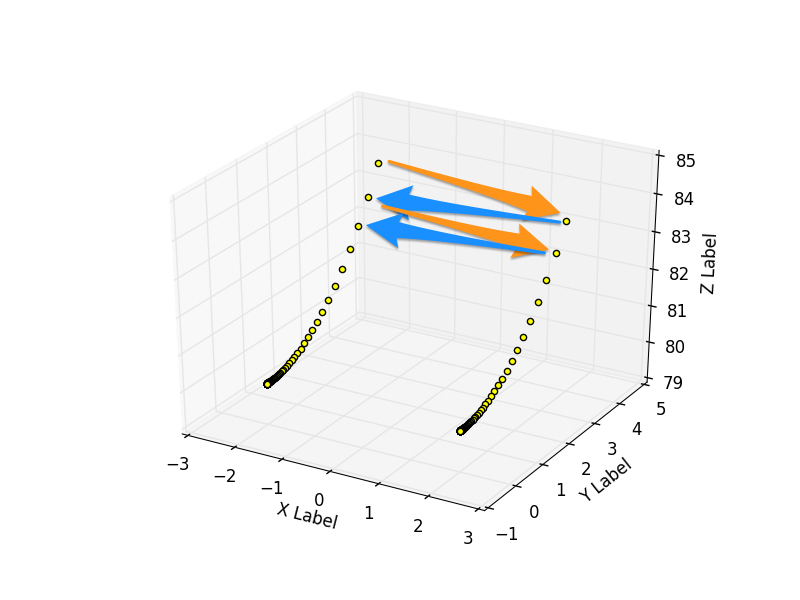
\includegraphics[width=300pt]{pictures/figure_1.png}
            \caption{gradient Descent with $\epsilon = 0.1$}
            \label{fig:fig1}
        \end{figure}
        as you can see in Figure \ref{fig:fig1} this is a very interesting special case because with this $\epsilon$ the gradient descent alternates between the ''sides'' (in respect to X) of our surface. This is caused by the derivative which is alternating between the same value positive and negative for the descent in direction X. So we are esentially endlessly looping in X-direction without any progress while only ``progressing'' in Y-direction. For every starting point there is exactly a \underline{single value} of $\epsilon$ which results in this behaviour. This result is caused by the symetry of our surface!
\end{enumerate}


\subsection{Numerical Computation 3}
\begin{enumerate}[a)]
    \item 
        see File
    \item
        % TODO
        TODO: Compare the path of finding the minimum to the one from exercise 3.
\end{enumerate}


\subsection{Numerical Computation 4}
% TODO
stop descent if one of these conditions hold:
\begin{itemize}
    \item 
        the derivative of f in this point is smaller than a chosen constant 0.0001 for 3 iterations in a row.
    \item
        we also stop in a special case just like in 2.3c by checking if we start alternating between 2 points. We could do this for example by storing the last 4 values for the derivative and checking if 
        $$ \text{dx}_0 - \text{dx}_2 \leq 0.0001 \quad \land \quad \text{dx}_1 - \text{dx}_3 \leq 0.0001 $$
\end{itemize}


\end{document}
